\documentclass[10pt,professionalfonts,serif,usenames,dvipsnames,svgnames,table]{beamer}

\usepackage{hyperref}
\hypersetup{
	pdfpagelabels=false
}

\usetheme{Warsaw}

\definecolor{darkgreen}{rgb}{0, 0.5, 0.0}
\newcommand{\docutilsrolegreen}[1]{\color{darkgreen}#1\normalcolor}
\newcommand{\docutilsrolered}[1]{\color{red}#1\normalcolor}

\newcommand{\green}[1]{\color{darkgreen}#1\normalcolor}
\newcommand{\red}[1]{\color{red}#1\normalcolor}

\usepackage{lmodern}
%\usepackage{garamond}
\usepackage[garamond]{mathdesign}
%\usepackage[urw-garamond]{mathdesign}

%\usepackage{amsmath}
%\usepackage{amssymb}
%\usepackage{amsthm}
%\usepackage{amsfonts}
\usepackage{graphicx}
\usepackage{verbatim}
\usepackage{fancyvrb}
\usepackage{verbments}
\usepackage{colortbl}
\usepackage{slashed}
\usepackage{tabularx}
%\usepackage[normalem]{ulem}
\usepackage{tikz}

\usepackage[loop, autoplay, buttonsize=1em, buttonbg=0, buttonfg=1]{animate}
\usepackage{movie15}

\providecommand\thispdfpagelabel[1]{}

\usetikzlibrary{shapes,arrows,trees}
\hypersetup{
colorlinks=true,
urlcolor=blue,
linkcolor=blue
}

%\usefonttheme[onlymath]{serif}
%\usecolortheme{orchid}
%\useinnertheme{rounded}

%\setbeamertemplate{headline}[default]
\setbeamercolor{author in head/foot}{fg=black,bg=white}
\setbeamercolor{title in head/foot}{fg=black,bg=white}
\setbeamercolor{date in head/foot}{fg=black,bg=white}

%\addtoheadtemplate{\pgfuseshading{beamer@headfade}\vskip-1.25cm}{}
%\usebackgroundtemplate{\includegraphics[width=\paperwidth,height=\paperheight]{images/bg.eps}}

%\setbeamercolor{frametitle}{bg=Blue,fg=white}
%\setbeamercolor{title}{bg=Blue,fg=white}

%\setbeamersize{text margin left=.2cm} 
%\setbeamersize{text margin right=.5cm}

\setbeamertemplate{itemize itemsep}[0.3in]
\setbeamertemplate{itemize parsep}[0.3in]
\setbeamertemplate{enumerate itemsep}[0.3in]
\setbeamertemplate{enumerate parsep}[0.3in]

\setbeamertemplate{navigation symbols}{}
\setbeamersize{text margin left=.2cm,text margin right=.2cm}
\setbeamercovered{transparent}

\newcommand{\maxFrameImage}[1]
{
	{
	\setbeamercolor{background canvas}{bg=black,fg=white}
	\usebeamercolor[fg]{background canvas}
	\begin{frame}[plain]
	\begin{changemargin}{-1cm}{-1cm}
	\begin{center}
	\includegraphics[width=1.01\paperwidth,height=1.01\paperheight,keepaspectratio]{#1}
	\end{center}
	\end{changemargin}
	\end{frame}
	}
}

\newenvironment{changemargin}[2]{
	\begin{list}{}
	{
	\setlength{\topsep}{-3pt}
	\setlength{\leftmargin}{#1}
	\setlength{\rightmargin}{#2}
	\setlength{\listparindent}{\parindent}
	\setlength{\itemindent}{\parindent}
	\setlength{\parsep}{\parskip}
	}
	\item[]
}{\end{list}}

\newenvironment<>{varblock}[2][\textwidth]
{
	\setlength{\textwidth}{#1}
	\begin{actionenv}#3
	\def\insertblocktitle{#2}
	\par
	\usebeamertemplate{block begin}
	}
	{\pa
	\usebeamertemplate{block end}
	\end{actionenv}
}

\defbeamertemplate*{footline}{my theme}
{
  \leavevmode%
  \hbox{%
  \begin{beamercolorbox}[wd=.333333\paperwidth,ht=3.25ex,dp=1.25ex,left]{author in head/foot}%
    \usebeamerfont{author in head/foot}\hspace*{3.25ex}\insertshortauthor~~(\insertshortinstitute)
  \end{beamercolorbox}%
  \begin{beamercolorbox}[wd=.333333\paperwidth,ht=3.25ex,dp=1.25ex,center]{date in head/foot}%
    \usebeamerfont{date in head/foot}%\insertshortdate{}\hspace*{2em}
    {\large\insertframenumber{}}/\inserttotalframenumber{}
  \end{beamercolorbox}}%
  \begin{beamercolorbox}[wd=.333333\paperwidth,ht=3.25ex,dp=1.25ex,right]{title in head/foot}%
    \usebeamerfont{title in head/foot}\insertshorttitle\hspace*{3.25ex}
  \end{beamercolorbox}%
  \vskip0pt%
}


../common/phys_defs.tex

\title{rootpy: Pythonic ROOT}
%\subtitle{I have no subtitle}
\author[Noel Dawe]{Noel Dawe}
\date[\today]{\today}
\institute[rootpy]{for the rootpy dev team}
\titlegraphic{\includegraphics[height=3cm]{../common/images/rootpy_logo.png}}

\begin{document}

\frame{\titlepage
    \begin{center}
    {\bf ROOT Users Workshop, Saas-Fee}
    \end{center}
}

\frame{
    \frametitle{``What's the problem?''}

    \begin{center}
    {\bf Why would we even consider developing a layer on top of PyROOT?}
    \end{center}

    \begin{itemize}
        \itemsep=.3cm
        \item PyROOT is mainly bindings (although with some pythonization).
        \item Python's dynamic nature provides {\bf many possibilities not
            currently realized by PyROOT}. One might argue a majority of these
            high-level pythonizations are {\bf beyond the scope of what PyROOT should
            offer.}
        \item Certain tasks require awkward code and are error-prone.
            Similar workarounds are implemented by many in multiple places.\\
            {\bf Why not solve these issues once and for all?}
        \item There is a lack of integration of ROOT with the vast and growing
            ecosystem of scientific Python packages.\\ {\bf Why not enable users to
            benefit from both the power of ROOT and what is offered by the
            scientific Python community?}
        \end{itemize}
}

\frame{
    \frametitle{Scientific Python Applications}
    \begin{center}
    ``Can I perform complicated analysis with Python?''\\
    {\bf You certainly can!}
    \end{center}
    \begin{itemize}
        \item \href{http://root.cern.ch/drupal/}{ROOT} with
            \href{http://root.cern.ch/drupal/content/pyroot}{PyROOT}
        \item Interactive computing: \href{http://ipython.org/}{IPython}
        \item Powerful and fast array manipulation:
            \href{http://numpy.scipy.org/}{NumPy}
        \item Efficiently and easily handle large amounts of data:
            \href{http://www.pytables.org/moin}{PyTables}
        \item General scientific library: \href{http://www.scipy.org/}{scipy}
        \item Data analysis and modeling: \href{http://pandas.pydata.org/}{pandas}
        \item Statistical models and tests: \href{http://statsmodels.sourceforge.net/}{statsmodels}
        \item Fitting: \href{http://cxc.harvard.edu/sherpa4.4/index.html}{sherpa}
        \item Astronomy: \href{http://www.astropy.org/}{astropy}
        \item Image processing: \href{http://scikit-image.org/}{scikit-image}
        \item Machine learning:
            \href{http://scikit-learn.org/stable/}{scikit-learn}
        \item Feature-rich publication-quality plotting:
            \href{http://matplotlib.org/}{matplotlib}
        \item See a list of other kits here:
            \href{http://scikits.appspot.com/scikits}{scikits.appspot.com/scikits}
    \end{itemize}
}

\frame{
    \frametitle{Introducing rootpy\ldots}

    \begin{itemize}
        \item rootpy aims to provide a \textbf{\emph{ more pythonic layer}} on
            top of the PyROOT bindings and to take advantage of advanced
            features of the Python language.
        \item {\bf rootpy does not intend to recreate ROOT} or to {\em severely}
            alter the default behaviour of ROOT.
        \item {\bf rootpy is not an analysis framework}, but rather a library that
            one's analysis framework might use.
        \item rootpy provides an {\bf interface with the scientific Python
            packages}:
        \end{itemize}
        \begin{center}
            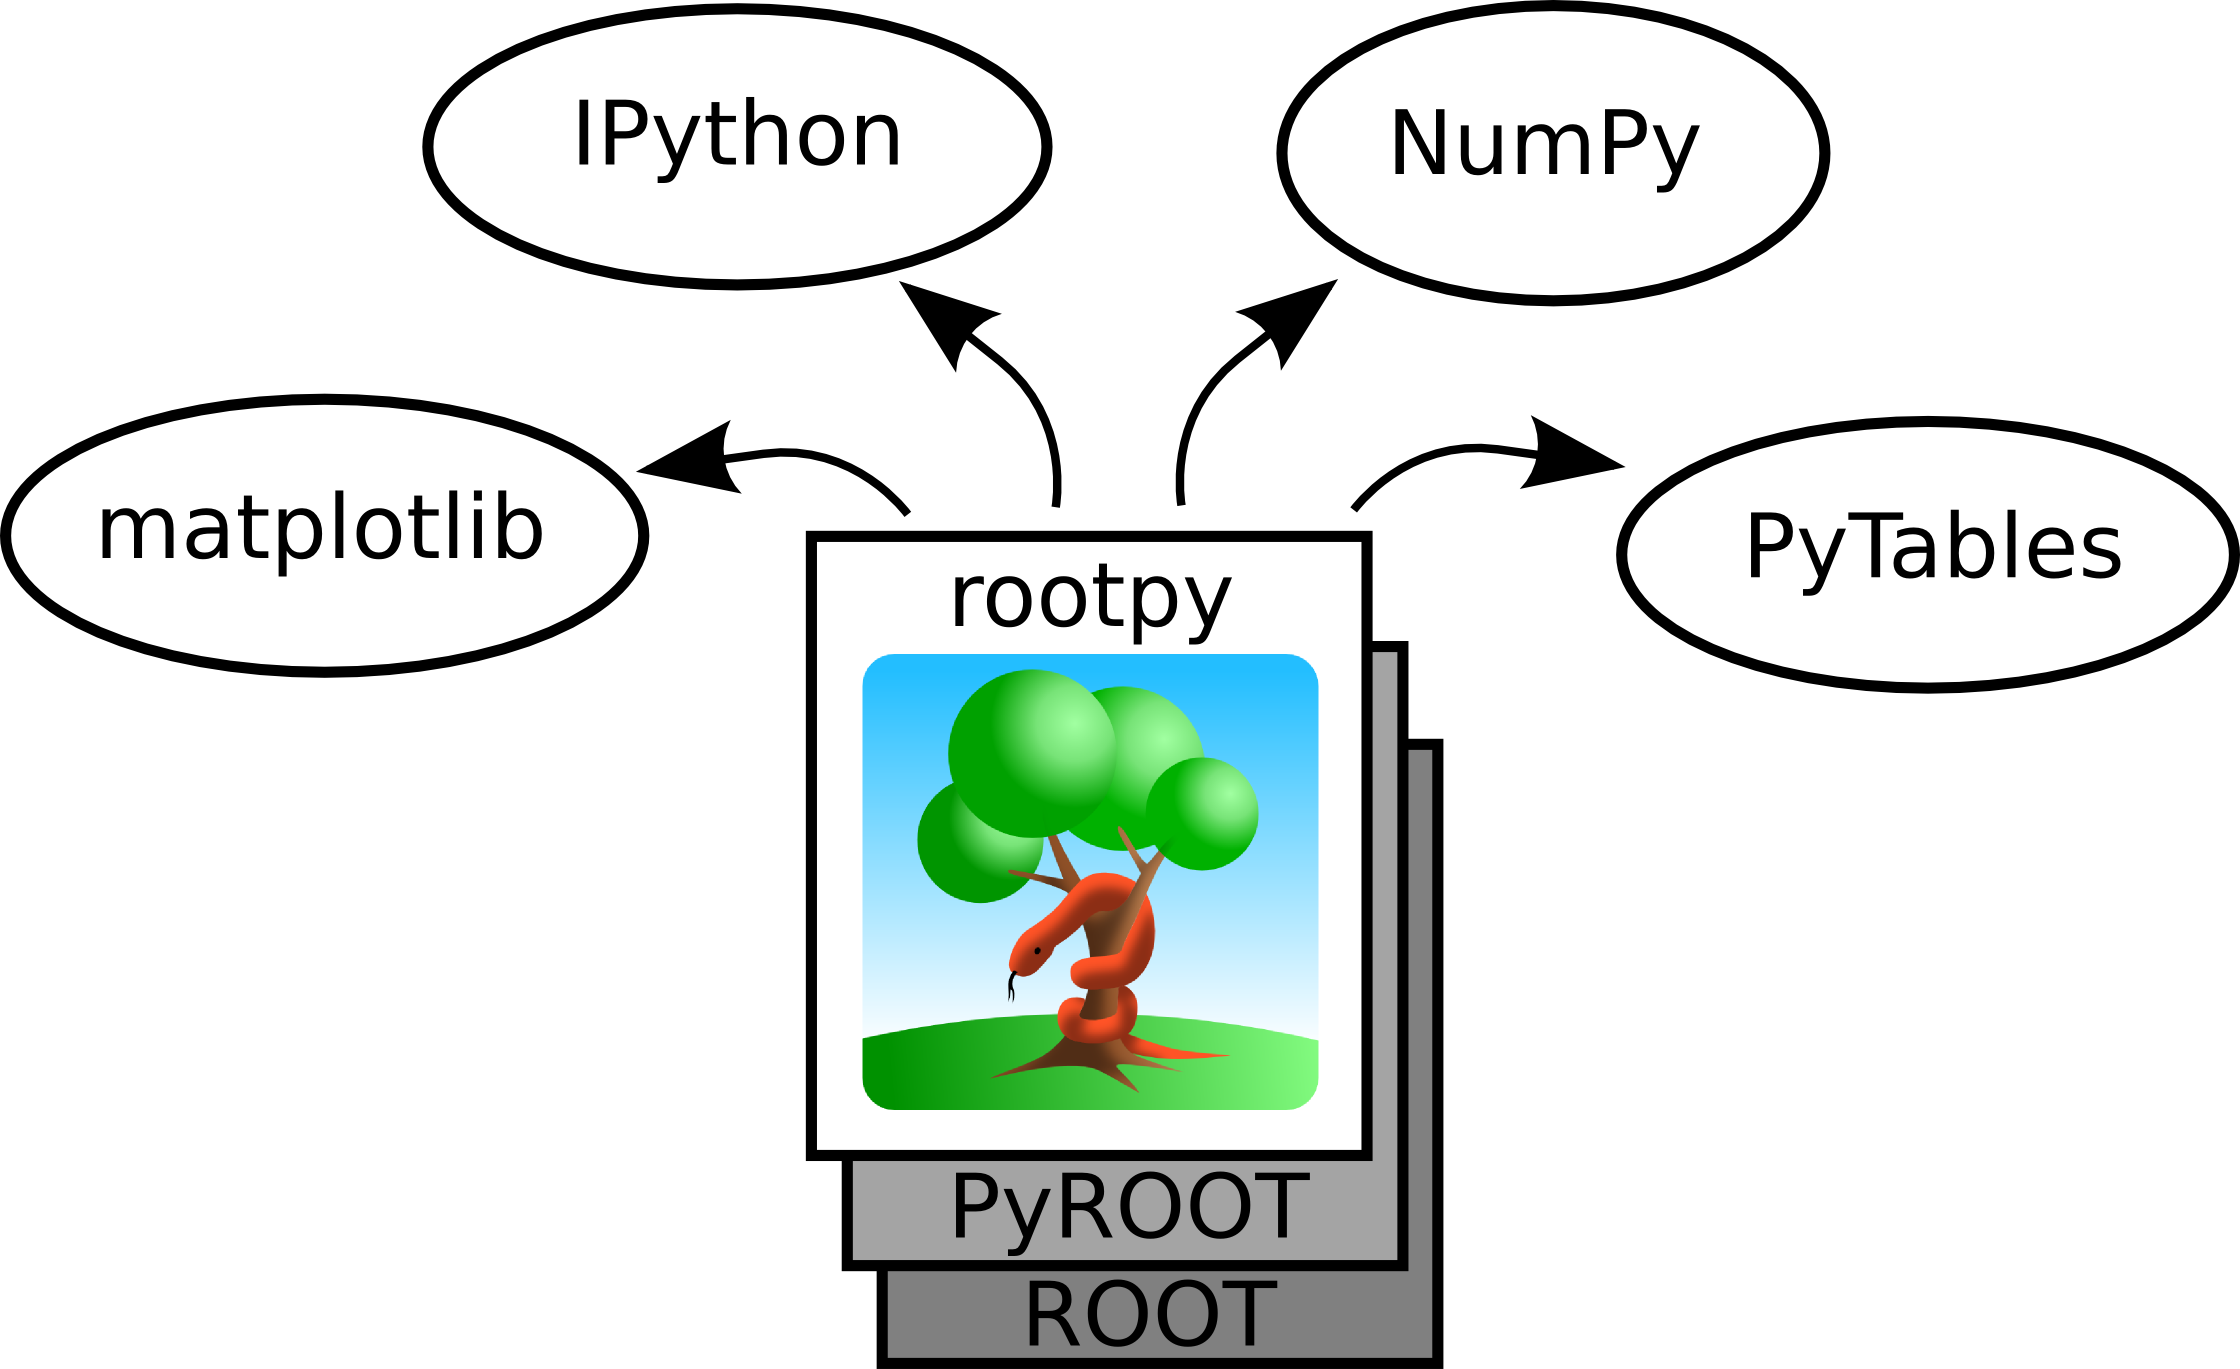
\includegraphics[width=.5\textwidth]{figs/rootpy-map.png}
        \end{center}
}

\frame{
    \frametitle{rootpy: key concepts and design philosophy}

    \begin{itemize}
        \itemsep=.3cm
        \item Pythonized {\bf classes in rootpy are subclasses of the corresponding
            ROOT classes} with the same (or similar) name, but without the ``T''.\\
        \item ROOT methods may be overridden or new methods created to add
            functionality and objects may be decorated with additional properties.
        \item {\bf Object names and titles are optional}. Unspecified names default to
            UUIDs.
        \item ROOT messages should be routed through Python's logging system
            with {\bf error messages raised as Python exceptions}.
        \item {\bf Python has a garbage collector but C++ does not:} this can lead to
            strange issues. rootpy addresses these problems.
        \item Anywhere Python is typically slow we intend to use
            {\bf compiled C extension modules}. Through the root\_numpy
            package, rootpy provides very fast conversion of ROOT Trees into
            NumPy arrays as well as efficiently filling ROOT histograms with
            NumPy arrays.
        \end{itemize}
}

\frame{
    \frametitle{``What does rootpy offer?''}

    \begin{center}
    \rowcolors[]{1}{blue!20}{blue!10}
    \begin{tabular}{l p{8cm}}
        {\bf rootpy.plotting} & histogram, graphs, canvas, pad, legend, and
            style subclasses with additional pythonizations,
            including a matplotlib interface. \\
        {\bf rootpy.tree} & trees, chains, tree objects, tree models, cuts. \\
        {\bf rootpy.io} & file and directory subclasses, utilities. \\
        {\bf rootpy.logger} & route ROOT messages through Python's
            logging module. ROOT error messages become Python exceptions. \\
        {\bf rootpy.memory} & utilities for monitoring TObject deletions
            and for keeping objects alive when out of scope in Python. \\
        {\bf rootpy.interactive} & a wait function for preventing Python
            from exiting until all canvases have been closed. \\
        {\bf rootpy.root2hdf5} & conversion of ROOT files to HDF5. \\
        {\bf rootpy.context} & utilities for managing ROOT's global state. \\
        \multicolumn{2}{c}{\ldots and more \ldots} \\
        \multicolumn{2}{c}{See the
            \href{https://github.com/rootpy/root\_numpy}{root\_numpy}
        package for conversion of TTrees into NumPy arrays.}\\
        \end{tabular}
    \end{center}
}

\begin{frame}[fragile]
    \frametitle{Histograms}
    {\bf PyROOT}
    \vspace{-.2cm}
    \begin{footnotesize}
\begin{pyglist}[language=python,texcl=true,abovecaptionskip=0,style=vs,bgcolor=Moccasin]
from ROOT import TH3D
from array import array

# variable width bins
hist3d = TH3D('3d', '3d', 3, array('d', [0, 3, 10, 100]),
                          5, array('d', [2.3, 4.2, 5.8, 10, 20, 25.5]),
                          2, array('d', [-100, 0, 20]))
# ROOT is missing some constructors... (the following will not work)
hist3d = TH3D('3d', '3d', 3, 0, 5,
                          5, array('d', [2.3, 4.2, 5.8, 10, 20, 25.5]),
                          2, array('d', [-100, 0, 20]))
\end{pyglist}
\end{footnotesize}

    {\bf rootpy}
    \vspace{-.2cm}
    \begin{footnotesize}
\begin{pyglist}[language=python,texcl=true,style=vs,bgcolor=Moccasin]
from rootpy.plotting import Hist3D

# variable width bins
hist3d = Hist3D([0, 3, 10, 100], [2.3, 4.2, 5.8, 10, 20, 25.5], [-100, 0, 20])
# easy to mix variable and fixed width bins with rootpy
hist3d = Hist3D(3, 0, 5, [2.3, 4.2, 5.8, 10, 20, 25.5], [-100, 0, 20])
\end{pyglist}
\end{footnotesize}

\end{frame}

\begin{frame}[fragile]
    \frametitle{Histograms and Style}
    \begin{itemize}
        \item rootpy reduces ROOT's histogram classes down to Hist, Hist2D,
            Hist3D.
        \item The appropriate ROOT base class is set {\em dynamically}:
            \begin{footnotesize}
\begin{pyglist}[language=python,texcl=true,style=vs]
>>> from rootpy.plotting import Hist2D
>>> hist = Hist2D(10, 0, 1, 5, 0, 1, type='F')
>>> hist.__class__.__bases__
(<class 'rootpy.plotting.hist._Hist2D'>, <class 'ROOT.TH2F'>)
\end{pyglist}
\end{footnotesize}
\item Attributes can be accessed via properties:
\begin{pyglist}[language=python,texcl=true,style=vs]
      hist.fillstyle = 'solid'
      color = hist.linecolor
\end{pyglist}
\item Colors can also be set using hex, RGB tuples, or SVG names:
\begin{pyglist}[language=python,texcl=true,style=vs]
      hist.fillcolor = (32, 178, 170)
      hist.linecolor = '#87cefa'
      hist.markercolor = 'salmon'
\end{pyglist}
\end{itemize}
\end{frame}

\begin{frame}[fragile]
    \frametitle{Cuts}
    \begin{columns}
        \column[t]{.45\textwidth}
        {\bf PyROOT}
        \begin{footnotesize}
\begin{pyglist}[language=python,texcl=true,style=vs,bgcolor=Moccasin]
from ROOT import TCut

cut1 = TCut('a<10')
cut2 = TCut('b%2==0')

cut = TCut('(%s)&&(%s)' % (cut1.GetTitle(), cut2.GetTitle()))
print cut.GetTitle()
\end{pyglist}
\end{footnotesize}

        output:
        \begin{footnotesize}
\begin{pyglist}[language=text,texcl=true,abovecaptionskip=0,style=bw]
(a<10)&&(b%2==0)
\end{pyglist}
\end{footnotesize}

        \column[t]{.45\textwidth}
        {\bf rootpy}
        \begin{footnotesize}
\begin{pyglist}[language=python,texcl=true,abovecaptionskip=0,style=vs,bgcolor=Moccasin]

cut1 = Cut('a < 10')
cut2 = Cut('b % 2 == 0')

cut = cut1 & cut2
print cut

# expansion of ternary conditions
cut3 = Cut('10 < a < 20')
print cut3

# easily combine cuts arbitrarily
cut = ((cut1 & cut2) | - cut3)
print cut
\end{pyglist}
\end{footnotesize}

        output:
        \begin{footnotesize}
\begin{pyglist}[language=text,texcl=true,abovecaptionskip=0,style=bw]
(a<10)&&(b%2==0)
(10<a)&&(a<20)
((a<10)&&(b%2==0))||(!((10<a)&&(a<20)))
\end{pyglist}
\end{footnotesize}

    \end{columns}
\end{frame}

\begin{frame}[fragile]
    \frametitle{PyROOT: Opening a TFile}

    \begin{footnotesize}
\begin{minted}{python}
"""
ROOT is unable to open the file of course and emits an error message but an
exception is not raised at this point leading to (sometimes difficult to
interpret) issues downstream:
"""
from ROOT import TFile

myfile = TFile.Open("file_does_not_exist.root")
print myfile
myfile.Get("something")
\end{minted}
\end{footnotesize}

    \vspace{-.5cm}
    \begin{footnotesize}
\begin{pyglist}[language=text,texcl=true,abovecaptionskip=0,style=bw]
Error in <TFile::TFile>: file file_does_not_exist.root does not exist
<ROOT.TFile object at 0x(nil)>
Traceback (most recent call last):
  File "file_open.py", line 6, in <module>
    myfile.Get("something")
ReferenceError: attempt to access a null-pointer
\end{pyglist}
\end{footnotesize}

\end{frame}

\begin{frame}[fragile]
    \frametitle{rootpy: Opening a TFile}

    \begin{footnotesize}
\begin{pyglist}[language=python,texcl=true,abovecaptionskip=0,style=vs,bgcolor=Moccasin]
from rootpy.io import root_open

myfile = root_open("file_does_not_exist.root")
print myfile
myfile.Get("something")
\end{pyglist}
\end{footnotesize}

    \vspace{-.5cm}
    \begin{footnotesize}
\begin{pyglist}[language=text,texcl=true,abovecaptionskip=0,style=bw]
ERROR:ROOT.TFile.TFile] file file_does_not_exist.root does not exist
Traceback (most recent call last):
  File "file_open_rootpy.py.tmp.py", line 13, in <module>
    myfile = root_open("file_does_not_exist.root")
  File "/home/endw/.local/lib/python2.7/site-packages/rootpy/io/file.py", line 224, in root_open
    root_file = ROOT.TFile.Open(filename, mode)
  File "/home/endw/.local/lib/python2.7/site-packages/rootpy/io/file.py", line 224, in root_open
    root_file = ROOT.TFile.Open(filename, mode)
  File "/home/endw/.local/lib/python2.7/site-packages/rootpy/logger/roothandler.py", line 91, in python_logging_error_handler
    raise ROOTError(level, location, msg)
rootpy.ROOTError: level=3000, loc='TFile::TFile', msg='file file_does_not_exist.root does not exist'
\end{pyglist}
\end{footnotesize}

\end{frame}

\begin{frame}[fragile]
    \frametitle{rootpy: Navigating a TFile}
    \begin{footnotesize}
\begin{minted}{python}
from rootpy.testdata import get_file

# use the test file shipped with rootpy
with get_file() as f:
    # access objects by name as properties of the current dir
    myhist = f.dimensions.hist2d
    # recursively walk through the file
    for path, dirs, objects in f.walk():
        # do something
        print path, dirs, objects
\end{minted}
\end{footnotesize}

    \vspace{-.5cm}
    \begin{footnotesize}
\begin{pyglist}[language=text,texcl=true,abovecaptionskip=0,style=bw]
 ['dimensions', 'scales', 'means', 'graphs', 'gaps', 'efficiencies'] []
dimensions [] ['hist2d', 'hist3d']
scales [] ['hist1', 'hist3', 'hist2', 'hist4']
means [] ['hist1', 'hist3', 'hist2', 'hist4']
graphs [] ['tgrapherrors', 'tgraph2d', 'tgraphasymmerrors', 'tgraph']
gaps [] ['hist1', 'hist3', 'hist2', 'hist4']
efficiencies [] ['hist1', 'hist3', 'hist2', 'hist4', 'eff3v1', 'eff2v1', 'eff4v1']
\end{pyglist}
\end{footnotesize}

\end{frame}

\begin{frame}[fragile]
    \frametitle{PyROOT: Filling a TTree}
    \begin{footnotesize}
\begin{pyglist}[language=python,texcl=true,abovecaptionskip=0,style=vs,bgcolor=Moccasin]
from array import array
from random import gauss

output_file = TFile.Open('output.root', 'recreate')
some_float = array('f', [0.])
some_int = array('i', [0])
tree = TTree('mytree', '')
tree.Branch('some_float', some_float, 'some_float/F')
tree.Branch('some_int', some_int, 'some_int/I')

for i in xrange(100):
    some_float[0] = gauss(0, 1)
    some_int[0] = i
    tree.Fill()

tree.Write()
output_file.Close()
\end{pyglist}
\end{footnotesize}

\end{frame}

\begin{frame}[fragile]
    \frametitle{rootpy: Filling a TTree}
    \begin{footnotesize}
\begin{pyglist}[language=python,texcl=true,abovecaptionskip=0,style=vs,bgcolor=Moccasin]
from rootpy.io import root_open as ropen
from random import gauss

f = ropen("test.root", "recreate")

tree = Tree("test")
tree.create_branches(
        {'x': 'F',
         'y': 'F',
         'z': 'F',
         'i': 'I'})

for i in xrange(10000):
    tree.x = gauss(.5, 1.)
    tree.y = gauss(.3, 2.)
    tree.z = gauss(13., 42.)
    tree.i = i
    tree.fill()
tree.write()
f.close()
\end{pyglist}
\end{footnotesize}

\end{frame}

\begin{frame}[fragile]
    \frametitle{rootpy: Tree Models}
    Easily create complex trees by simple class inheritance (inspired by
    PyTables):
    \vspace{-.5cm}
    \begin{columns}
        \column[t]{.45\textwidth}
    \begin{footnotesize}
\begin{minted}{python}
from rootpy.tree import Tree
from rootpy.tree import TreeModel
from rootpy.types import FloatCol
from rootpy.types import IntCol

class FourVect(TreeModel):
    eta = FloatCol(default=-1111.)
    phi = FloatCol(default=-1111.)
    pt = FloatCol()
    m = FloatCol()

class Tau(FourVect):
    numtrack = IntCol()

class Event(Tau.prefix('tau1_'),
            Tau.prefix('tau2_')):
    event_number = IntCol()
    run_number = IntCol()

# tree = Tree('data', model=Event)
print Event
\end{minted}
\end{footnotesize}

    \column[t]{.45\textwidth}
    \begin{footnotesize}
\begin{minted}{text}
tau1_eta -> FloatCol(default=-1111.0)
tau2_eta -> FloatCol(default=-1111.0)
tau1_phi -> FloatCol(default=-1111.0)
tau2_phi -> FloatCol(default=-1111.0)
tau1_pt -> FloatCol()
tau2_pt -> FloatCol()
tau1_m -> FloatCol()
tau2_m -> FloatCol()
tau1_numtrack -> IntCol()
tau2_numtrack -> IntCol()
event_number -> IntCol()
run_number -> IntCol()
\end{minted}
\end{footnotesize}

    \end{columns}
\end{frame}

\begin{frame}[fragile]
    \frametitle{Memory issues? Solved.}
    \begin{columns}
        \column[t]{.45\textwidth}
        {\bf PyROOT}
    \begin{footnotesize}
\begin{minted}{python}
from ROOT import TCanvas, TH1D

def make_plot():
    canvas = TCanvas('plot', 'plot',
                     700, 500)
    hist = TH1D('hist', 'plot',
                10, -3, 3)
    hist.FillRandom('gaus')
    hist.Draw()
    return canvas

canvas = make_plot()
# empty canvas since the histogram
# has been garbage collected!
canvas.Draw()
# hack to keep Python from exiting
# while the canvas is displayed
raw_input()
\end{minted}
\end{footnotesize}

        \column[t]{.45\textwidth}
        {\bf rootpy}
    \begin{footnotesize}
\begin{pyglist}[language=python,texcl=true,abovecaptionskip=0,style=vs,bgcolor=Moccasin]
from rootpy.plotting import Canvas, Hist
from rootpy.interactive import wait

def make_plot():
    canvas = Canvas(700, 500)
    hist = Hist(10, -3, 3)
    hist.FillRandom('gaus')
    hist.Draw()
    return canvas

canvas = make_plot()
canvas.Draw()
wait()
\end{pyglist}
\end{footnotesize}

    Objects are kept alive as long as the Canvas is alive. \\
    {\bf See rootpy's keepalive function.}
    \end{columns}
\end{frame}

\begin{frame}
    \frametitle{rootpy: Interface with matplotlib}
    ROOT histograms
    \href{https://github.com/rootpy/rootpy/blob/master/examples/plotting/plot_matplotlib_hist.py}{
    can be drawn with matplotlib} via rootpy's
    \href{https://github.com/rootpy/rootpy/blob/master/rootpy/plotting/root2matplotlib.py}{
    matplotlib interface}:
    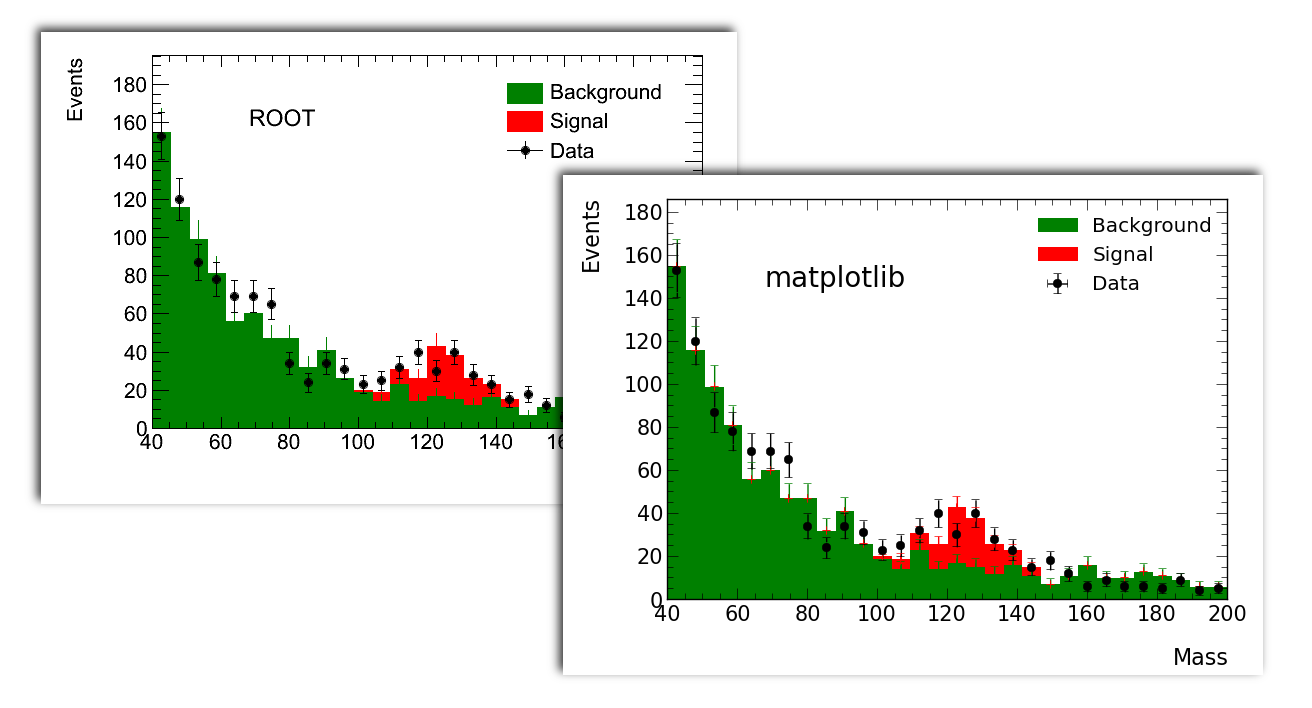
\includegraphics[width=\textwidth]{figs/examples/matplotlib_example.png}
\end{frame}


\frame{
    \frametitle{The future of rootpy}

    \begin{itemize}
        \item Benefit from ROOT 6!
        \item Larger documentation coverage and more examples. {\bf This is important!}
        \item Python 3 support.
        \item Better integration with the IPython prompt:
            \begin{itemize}
                \item Full tab completion and helpful builtin commands like pylab.
                \item Fetch documentation on-demand for a class/method/function.
                \end{itemize}
        \item Automatic wrapping of ROOT methods by parsing method signatures:
            \begin{itemize}
                \item If a method expects a TColor, rootpy can accept any matplotlib/ROOT color
                      and convert it into a TColor before passing to the ROOT method.
                \item Reduce the amount of code in rootpy.
                \end{itemize}
       \item TMVA:
           \begin{itemize}
                \item Ability to feed TMVA classifiers NumPy arrays.
                \end{itemize}
       \item RooFit and RooStats:
           \begin{itemize}
                \item Wrap RooArgSet as set() and RooArgList as list()?
                \item Create RooDataSets from NumPy arrays.
                \end{itemize}
       \item rootpy should serve as a {\bf testing ground for new ideas}.
   \end{itemize}
}

\begin{frame}[fragile]
    \frametitle{``How do I install rootpy?''}
    \begin{enumerate}
        \item First install ROOT with python support enabled (PyROOT)
        \item Clone the rootpy repository with git:
\begin{pyglist}[language=bash,texcl=true,style=vim]
git clone git://github.com/rootpy/rootpy.git
\end{pyglist}
        \item or checkout with svn:
\begin{pyglist}[language=bash,texcl=true,style=vim]
svn checkout http://svn.github.com/rootpy/rootpy
\end{pyglist}
        \item Then install:
\begin{pyglist}[language=bash,texcl=true,style=vim]
cd rootpy
python setup.py install --user
\end{pyglist}
\end{enumerate}
\begin{itemize}
    \item or install a \href{https://pypi.python.org/pypi/rootpy}{released version}
        with \href{https://pypi.python.org/pypi/pip}{pip}:
\begin{pyglist}[language=bash,texcl=true,style=vim]
pip install --user rootpy
\end{pyglist}
        \item See the
                \href{https://github.com/rootpy/rootpy/blob/master/README.rst}{README}
                for full instructions.
    \end{itemize}
\end{frame}

\begin{frame}[fragile]
    \frametitle{How can you contribute?}

    \begin{center}
    
\includegraphics[width=5cm]{figs/we-want-you.jpg}
    \end{center}

    \begin{itemize}
        \item Development is community-driven.
        \item We use Git! See the rootpy collaboration on GitHub:
            \href{https://github.com/rootpy}{github.com/rootpy}
        \item Just fork rootpy into your own GitHub account and:
            \begin{pyglist}[language=bash,texcl=true,style=vim]
git clone git@github.com:<username>/rootpy.git
            \end{pyglist}
              Then submit a pull request with your contribution.
        \item Contributions are reviewed by peers before merging into the main branch.
        \item All new code automatically triggers our test suite using
            \href{https://travis-ci.org/}{Travis CI}.
    \end{itemize}
\end{frame}

\begin{frame}
    \begin{large}
    \begin{center}
    \begin{columns}
        \column[t]{.35\textwidth}
{\bf The Developers:}
\vspace{.5cm}
\begin{itemize}
    \item Noel Dawe
    \item Peter Waller
    \item Evan Friis
    \item Christoph Deil
    \item Jeff Klukas
    \item Alessandro Thea
    \item Jeroen Hegeman
\end{itemize}
\column[t]{.35\textwidth}
{\bf Where to find us:}
\vspace{.5cm}
        \begin{itemize}
            \item \href{http://rootpy.org}{rootpy.org}
            \item \href{https://github.com/rootpy}{github.com/rootpy}
            \item \href{http://www.ohloh.net/p/rootpy}{ohloh.net/p/rootpy}
            \item \href{http://webchat.freenode.net/?randomnick=1&channels=rootpy&prompt=1}{IRC}
            \end{itemize}
        \end{columns}
    \end{center}
    \end{large}
\end{frame}

\end{document}
